%%%%%%%%%%%%%%%%%%%%%%%%%%%%%%%%%%%%%%%%%
% Beamer Presentation
% LaTeX Template
% Version 1.0 (10/11/12)
%
% This template has been downloaded from:
% http://www.LaTeXTemplates.com
%
% License:
% CC BY-NC-SA 3.0 (http://creativecommons.org/licenses/by-nc-sa/3.0/)
%
%%%%%%%%%%%%%%%%%%%%%%%%%%%%%%%%%%%%%%%%%

%----------------------------------------------------------------------------------------
%	PACKAGES AND THEMES
%----------------------------------------------------------------------------------------

\documentclass{beamer}

\mode<presentation> {

% The Beamer class comes with a number of default slide themes
% which change the colors and layouts of slides. Below this is a list
% of all the themes, uncomment each in turn to see what they look like.

%\usetheme{default}
%\usetheme{AnnArbor}
%\usetheme{Antibes}
%\usetheme{Bergen}
%\usetheme{Berkeley}
%\usetheme{Berlin}
%\usetheme{Boadilla}
%\usetheme{CambridgeUS}
%\usetheme{Copenhagen}
%\usetheme{Darmstadt}
%\usetheme{Dresden}
%\usetheme{Frankfurt}
%\usetheme{Goettingen}
%\usetheme{Hannover}
%\usetheme{Ilmenau}
%\usetheme{JuanLesPins}
%\usetheme{Luebeck}
\usetheme{Madrid}
%\usetheme{Malmoe}
%\usetheme{Marburg}
%\usetheme{Montpellier}
%\usetheme{PaloAlto}
%\usetheme{Pittsburgh}
%\usetheme{Rochester}
%\usetheme{Singapore}
%\usetheme{Szeged}
%\usetheme{Warsaw}

% As well as themes, the Beamer class has a number of color themes
% for any slide theme. Uncomment each of these in turn to see how it
% changes the colors of your current slide theme.

%\usecolortheme{albatross}
%\usecolortheme{beaver}
%\usecolortheme{beetle}
%\usecolortheme{crane}
%\usecolortheme{dolphin}
%\usecolortheme{dove}
%\usecolortheme{fly}
%\usecolortheme{lily}
%\usecolortheme{orchid}
%\usecolortheme{rose}
%\usecolortheme{seagull}
%\usecolortheme{seahorse}
%\usecolortheme{whale}
%\usecolortheme{wolverine}

%\setbeamertemplate{footline} % To remove the footer line in all slides uncomment this line
%\setbeamertemplate{footline}[page number] % To replace the footer line in all slides with a simple slide count uncomment this line

%\setbeamertemplate{navigation symbols}{} % To remove the navigation symbols from the bottom of all slides uncomment this line
}

\usepackage{graphicx} % Allows including images
\usepackage{booktabs} % Allows the use of \toprule, \midrule and \bottomrule in tables
\usepackage{tikz}
\usepackage{tikz-network}
%----------------------------------------------------------------------------------------
%	TITLE PAGE
%----------------------------------------------------------------------------------------

\title[Diffusion Auction in Social Networks]{Diffusion Auction in Social Networks} % The short title appears at the bottom of every slide, the full title is only on the title page

\author{Five Minutes Research Presentation} % Your name
\institute[] % Your institution as it will appear on the bottom of every slide, may be shorthand to save space
{
%University of California \\ % Your institution for the title page
\medskip
\textit{} % Your email address
}
\date{} % Date, can be changed to a custom date

\begin{document}

\begin{frame}
\titlepage % Print the title page as the first slide
\end{frame}

%\begin{frame}
%\frametitle{Overview} % Table of contents slide, comment this block out to remove it
%\tableofcontents % Throughout your presentation, if you choose to use \section{} and \subsection{} commands, these will automatically be printed on this slide as an overview of your presentation
%\end{frame}

%----------------------------------------------------------------------------------------
%	PRESENTATION SLIDES
%----------------------------------------------------------------------------------------

%------------------------------------------------
%\section{First Section} % Sections can be created in order to organize your presentation into discrete blocks, all sections and subsections are automatically printed in the table of contents as an overview of the talk
%------------------------------------------------

%\subsection{Subsection Example} % A subsection can be created just before a set of slides with a common theme to further break down your presentation into chunks

\begin{frame}
\frametitle{Introduction: How can you sell a commodity?}


\begin{block}{Traditional Approaches}
\begin{itemize}
\item Contacting some on-line sales platform
\item Using ads via some social media 
\end{itemize}
\end{block}
\begin{alertblock}{Challenge}
\begin{itemize}
\item \alert{Unpredictable} returns, suffer from \alert{DEFICIT}!
\item Attract more people while guarantee  profits.
\end{itemize}
\end{alertblock}
\begin{figure}
\centering

\includegraphics[height=1cm]{downarrow.pdf}
\end{figure}
\begin{center}
\Large{\textbf{Selling a commodity via social network!}}
\end{center}
\end{frame}

%------------------------------------------------

\begin{frame}
\frametitle{Diffusion Auction Settings}
%插一个网络图
\begin{columns}
\begin{column}{.4\linewidth}
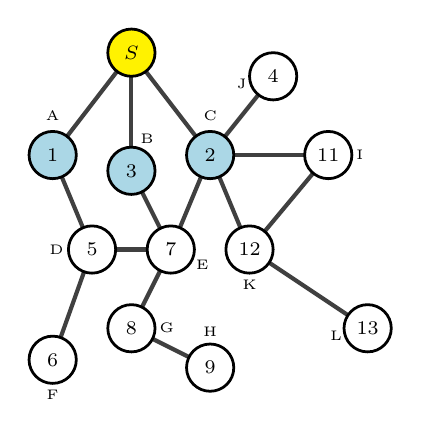
\begin{tikzpicture}
\Vertex[x=2,y=4.5,color=yellow,label=$S$]{S}
\Vertex[x=1,y=3.2,label=$1$]{A}
\Vertex[x=2,y=3,label=$3$]{B}
\Vertex[x=3,y=3.2,label=$2$]{C}
\Vertex[x=1.5,y=2,color=white,label=$5$]{D}
\Vertex[x=2.5,y=2,color=white,label=$7$]{E}
\Vertex[x=1,y=0.6,color=white,label=$6$]{F}
\Vertex[x=2,y=1,color=white,label=$8$]{G}
\Vertex[x=3,y=0.5,color=white,label=$9$]{H}
\Vertex[x=4.5,y=3.2,color=white,label=$11$]{I}
\Vertex[x=3.8,y=4.2,color=white,label=$4$]{J}
\Vertex[x=3.5,y=2,color=white,label=$12$]{K}
\Vertex[x=5,y=1,color=white,label=\alert{13}]{L}
\Text[x=1,y=3.7,fontsize=\tiny]{A}
\Text[x=2.2,y=3.4,fontsize=\tiny]{B}
\Text[x=3,y=3.7,fontsize=\tiny]{C}
\Text[x=1.05,y=2,fontsize=\tiny]{D}
\Text[x=2.9,y=1.8,fontsize=\tiny]{E}
\Text[x=1,y=0.15,fontsize=\tiny]{F}
\Text[x=2.45,y=1,fontsize=\tiny]{G}
\Text[x=3,y=0.95,fontsize=\tiny]{H}
\Text[x=4.9,y=3.2,fontsize=\tiny]{I}
\Text[x=3.4,y=4.1,fontsize=\tiny]{J}
\Text[x=3.5,y=1.55,fontsize=\tiny]{K}
\Text[x=4.6,y=0.9,fontsize=\tiny]{L}
\Edge[](S)(A)
\Edge[](S)(B)
\Edge[](S)(C)
\Edge[](A)(D)
\Edge[](B)(E)
\Edge[](D)(F)
\Edge[](D)(E)
\Edge[](C)(E)
\Edge[](E)(G)
\Edge[](G)(H)
\Edge[](C)(J)
\Edge[](C)(I)
\Edge[](C)(K)
\Edge[](K)(L)
\Edge[](K)(I)
\end{tikzpicture}
\end{column}

\begin{column}{.6\linewidth}
\begin{itemize}
\item Seller $s$ sells a commodity.
\item Having contact with neighbour nodes.
\item (Without diffusion) Seller $s$ sells the item among A,B,C.
\item Competition $\Rightarrow$ \textbf{Nobody diffuse!}
\end{itemize}
\begin{figure}
\centering

\includegraphics[height=0.8cm]{downarrow.pdf}
\end{figure}
\begin{itemize}
\item \textbf{Target 1}: Encouraging Diffusion!
\item \textbf{Target 2}: Encouraging Truthful Bid!
\end{itemize}
\end{column}
\end{columns}
\end{frame}

%------------------------------------------------

\begin{frame}
\frametitle{New Mechanism: Information Diffusion Mechanism}
\begin{columns}
\begin{column}{.4\linewidth}
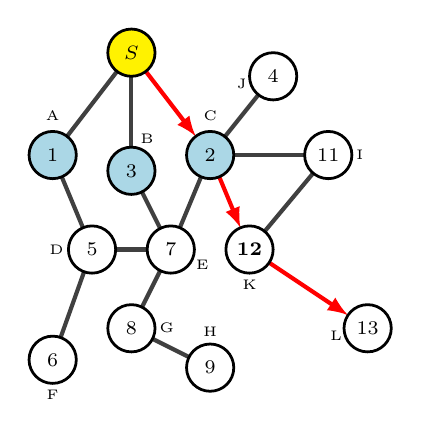
\begin{tikzpicture}
\Vertex[x=2,y=4.5,color=yellow,label=$S$]{S}
\Text[x=1,y=3.7,fontsize=\tiny]{A}
\Vertex[x=1,y=3.2,label=$1$]{A}
\Text[x=2.2,y=3.4,fontsize=\tiny]{B}
\Vertex[x=2,y=3,label=$3$]{B}
\Text[x=3,y=3.7,fontsize=\tiny]{C}
\Vertex[x=3,y=3.2,label=$2$]{C}
\Text[x=1.05,y=2,fontsize=\tiny]{D}
\Vertex[x=1.5,y=2,color=white,label=$5$]{D}
\Text[x=2.9,y=1.8,fontsize=\tiny]{E}
\Vertex[x=2.5,y=2,color=white,label=$7$]{E}
\Text[x=1,y=0.15,fontsize=\tiny]{F}
\Vertex[x=1,y=0.6,color=white,label=$6$]{F}
\Text[x=2.45,y=1,fontsize=\tiny]{G}
\Vertex[x=2,y=1,color=white,label=$8$]{G}
\Text[x=3,y=0.95,fontsize=\tiny]{H}
\Vertex[x=3,y=0.5,color=white,label=$9$]{H}
\Text[x=4.9,y=3.2,fontsize=\tiny]{I}
\Vertex[x=4.5,y=3.2,color=white,label=$11$]{I}
\Text[x=3.4,y=4.1,fontsize=\tiny]{J}
\Vertex[x=3.8,y=4.2,color=white,label=$4$]{J}
\Text[x=3.5,y=1.55,fontsize=\tiny]{K}
\Vertex[x=3.5,y=2,color=white,label=\alert{\textbf{12}}]{K}
\Text[x=4.6,y=0.9,fontsize=\tiny]{L}
\Vertex[x=5,y=1,color=white,label=13]{L}
\Edge[](S)(A)
\Edge[](S)(B)
\Edge[color=red,Direct=True](S)(C)
\Edge[](A)(D)
\Edge[](B)(E)
\Edge[](D)(F)
\Edge[](D)(E)
\Edge[](C)(E)
\Edge[](E)(G)
\Edge[](G)(H)
\Edge[](C)(J)
\Edge[](C)(I)
\Edge[color=red,Direct=True](C)(K)
\Edge[color=red,Direct=True](K)(L)
\Edge[](K)(I)
\end{tikzpicture}
Final winner is \alert{K}; \\Rewarded bidder: \textcolor{blue}{C}.
\end{column}
\begin{column}{.6\linewidth}
%\begin{definition}[Critical Diffusion Node]
%$i$ is $j$'s critical diffusion node if all the diffusion paths started from seller to $j$ have to pass $i$. 
%\end{definition}
\begin{itemize}
\item Critical Diffusion Nodes \& Sequence.
\item Allocation Rule:
\[
\pi_i^{idm}=
\begin{cases}
1&i\in C_m\backslash \{m\},v_i=v^\ast_{-d_{i+1}}\\
1& i=m\\
0&\text{otherwise}
\end{cases}
\]
\item Payment Rule:
\[
p_i^{idm}=
\begin{cases}
v^\ast_{-d_i}-v^\ast_{d_{i+1}}&i\in C_w\backslash \{w\}\\
v^\ast_{-d_i}& i=w\\
0&\text{otherwise}
\end{cases}
\]
\item Truthful bid and propagation!
\end{itemize}
\end{column}
\end{columns}
\end{frame}

%------------------------------------------------

\begin{frame}
\frametitle{Conclusion And Discussion}
\begin{block}{Conclusions}
\begin{enumerate}
\item Generalizing classical auction into a social network.
\item Encouraging bidders propagating sale information to neighbours.
\item Getting higher profit for both seller and bidders.
\end{enumerate}
\end{block}
\begin{block}{Future of Diffusion Auction}
\begin{enumerate}

\item Maximizing the seller's revenue.
\item Considering different social networks' impacts.
\item Extending to multiple items auction.
\end{enumerate}
\end{block}
\begin{center}
\Large{\textbf{Thanks for listening!}}
\end{center}
\end{frame}
%------------------------------------------------

%------------------------------------------------

%------------------------------------------------

%------------------------------------------------

%------------------------------------------------

%------------------------------------------------

%----------------------------------------------------------------------------------------

\end{document} 